\documentclass[border=4pt]{standalone}
\usepackage{fontspec}
\usepackage{amsmath}
\usepackage{unicode-math}
\setmainfont{Latin Modern Roman}
\setmathfont{Latin Modern Math}
\usepackage{pgfplots}
\usepackage{pgfplotstable}
\pgfplotsset{compat=1.18}
\usepackage{tkz-euclide}
\usetikzlibrary{arrows.meta,calc,angles,quotes,patterns,3d,backgrounds}
\definecolor{ink}{HTML}{123428}
\definecolor{asy}{HTML}{475569}
\definecolor{mint}{HTML}{86e0bd}
\tikzset{asym/.style={asy, line width=0.9pt, dash pattern=on 5pt off 3.5pt},
         guide/.style={gray!70, line width=0.6pt, densely dotted},
         dot/.style={circle, inner sep=0pt, minimum size=5pt, draw=white, line width=0.5pt},
         odot/.style={circle, inner sep=0pt, minimum size=5.5pt, fill=white, line width=1pt},
         lab/.style={font=\footnotesize, inner sep=1.5pt, text=ink}}
\begin{document}
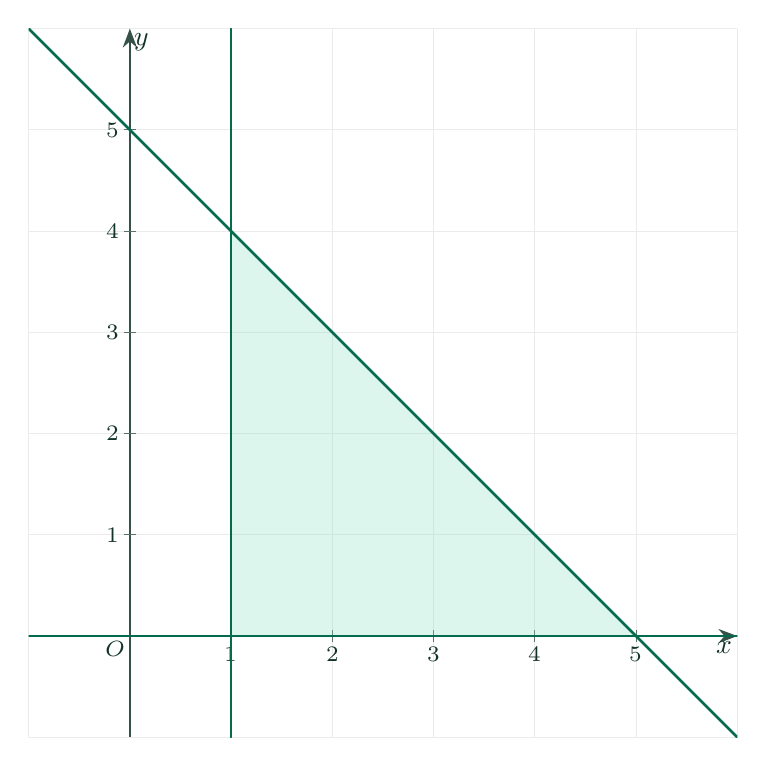
\begin{tikzpicture}[x=1.2857cm, y=1.2857cm]
\draw[gray!16, line width=0.4pt] (-1,-1) -- (-1,6) (0,-1) -- (0,6) (1,-1) -- (1,6) (2,-1) -- (2,6) (3,-1) -- (3,6) (4,-1) -- (4,6) (5,-1) -- (5,6) (6,-1) -- (6,6);
\draw[gray!16, line width=0.4pt] (-1,-1) -- (6,-1) (-1,0) -- (6,0) (-1,1) -- (6,1) (-1,2) -- (6,2) (-1,3) -- (6,3) (-1,4) -- (6,4) (-1,5) -- (6,5) (-1,6) -- (6,6);
\draw[ink!85, line width=0.7pt, -{Stealth[length=2.4mm]}] (-1,0) -- (6,0) node[anchor=north east, lab, font=\normalsize] {$x$};
\draw[ink!85, line width=0.7pt, -{Stealth[length=2.4mm]}] (0,-1) -- (0,6) node[anchor=north west, lab, font=\normalsize] {$y$};
\draw[ink!70] (1,0.06222222222222222) -- (1,-0.06222222222222222) node[below, lab, font=\footnotesize] {$1$};
\draw[ink!70] (2,0.06222222222222222) -- (2,-0.06222222222222222) node[below, lab, font=\footnotesize] {$2$};
\draw[ink!70] (3,0.06222222222222222) -- (3,-0.06222222222222222) node[below, lab, font=\footnotesize] {$3$};
\draw[ink!70] (4,0.06222222222222222) -- (4,-0.06222222222222222) node[below, lab, font=\footnotesize] {$4$};
\draw[ink!70] (5,0.06222222222222222) -- (5,-0.06222222222222222) node[below, lab, font=\footnotesize] {$5$};
\draw[ink!70] (0.06222222222222222,1) -- (-0.06222222222222222,1) node[left, lab, font=\footnotesize] {$1$};
\draw[ink!70] (0.06222222222222222,2) -- (-0.06222222222222222,2) node[left, lab, font=\footnotesize] {$2$};
\draw[ink!70] (0.06222222222222222,3) -- (-0.06222222222222222,3) node[left, lab, font=\footnotesize] {$3$};
\draw[ink!70] (0.06222222222222222,4) -- (-0.06222222222222222,4) node[left, lab, font=\footnotesize] {$4$};
\draw[ink!70] (0.06222222222222222,5) -- (-0.06222222222222222,5) node[left, lab, font=\footnotesize] {$5$};
\node[lab, anchor=north east] at (0,0) {$O$};
\tkzDefPoint(1,4){tmp1}
\tkzDefPoint(1,0){tmp2}
\tkzDefPoint(5,0){tmp3}
\tkzDefPoint(1,-1){tmp4}
\tkzDefPoint(1,6){tmp5}
\tkzDefPoint(6,0){tmp6}
\tkzDefPoint(-1,0){tmp7}
\tkzDefPoint(-1,6){tmp8}
\tkzDefPoint(6,-1){tmp9}
\begin{scope}
\clip (-1,-1) rectangle (6,6);
\tkzFillPolygon[fill={rgb,255:red,134;green,224;blue,189}, fill opacity=0.28](tmp1,tmp2,tmp3)
\tkzDrawSegment[draw={rgb,255:red,4;green,107;blue,77}, line width=0.90pt](tmp4,tmp5)
\tkzDrawSegment[draw={rgb,255:red,4;green,107;blue,77}, line width=0.90pt](tmp6,tmp7)
\tkzDrawSegment[draw={rgb,255:red,4;green,107;blue,77}, line width=0.90pt](tmp8,tmp9)
\end{scope}
\end{tikzpicture}
\end{document}
